%\section{Anforderungen}
%\textit{In diesem Abschnitt soll die Demoanwendung vorgestellt werden, anhand dessen das Proof-of-Concept erstellt wird. Damit das Proof-of-Concept erstellt werden kann, muss die Demoanwendung die zuvor beschriebenen Probleme aufweisen, hierbei sollen die Probleme möglichst realitätsnah sein und nicht frei erfunden.}

Wie in \autoref{anf:1020} beschrieben, ist eine Demoanwendung zu erstellen, auf Basis dessen das Konzept anzuwenden ist und somit praktisch umgesetzt werden kann. Dieser Abschnitt beschäftigt sich mit der Vorstellung der Demoanwendung und der repräsentativen Aufgabe, die diese übernimmt.

In der Motivation wurde ein konkretes Problem eines Kunden der Open Knowledge genannt. Damit die Demoanwendung realistisch eine , wird sie in Grundzügen die Webanwendung des Direktversicherers nachahmen. Bei der Webanwendung handelt es sich um eine mit Angular erstellte SPA, die den Nutzer verschiedene teils dynamische Formulare ausfüllen lässt und am Ende diese Daten an einen Dienst sendet und ein Ergebnis erhält, welches dargestellt wird. Während der Eingabe der Formulare werden einzelne Werte gegen Dienste validiert. Um die gewünschte Demoanwendung zu definieren, wird im folgenden Abschnitt das Verhalten festgelegt.

\subsection{Verhaltensdefinition}

Mit den beiden Stakeholdern, also Christian Wansart und Stephan Müller, die beide am Projekt für den Kunden involviert sind, wurde diese Verhaltensdefinition erstellt. Diesen Ansatz der Definition der Software anhand des Verhaltens nennt man Behavior Driven Development (BDD). Um die BDD-Definition festzuhalten wurde sie in der gängigen Gherkin \cite{Gherkin} Syntax geschrieben. Die Syntax ist natürlich zu lesen, und folgend werden alle gewünschen Features der Demoanwendung in der Gherkin-Syntax beschrieben.

\lstinputlisting[
  language = gherkin,
   caption = Demoanwendung: Gherkin Definition zum Feature \enquote{Warenkorb},
captionpos = b,
     label = lst:demoanwendung-gherkin-warenkorb
]{content/04_erstellung-poc/warenkorb-gherkin/1-warenkorb.feature}

\lstinputlisting[
  language = gherkin,
   caption = Demoanwendung: Gherkin Definition zum Feature \enquote{Rechnungsadresse},
captionpos = b,
     label = lst:demoanwendung-gherkin-rechnungsadresse
]{content/04_erstellung-poc/warenkorb-gherkin/2-rechnungsadresse.feature}

\lstinputlisting[
  language = gherkin,
   caption = Demoanwendung: Gherkin Definition zum Feature \enquote{Lieferadresse},
captionpos = b,
     label = lst:demoanwendung-gherkin-lieferadresse
]{content/04_erstellung-poc/warenkorb-gherkin/3-lieferadresse.feature}

\lstinputlisting[
  language = gherkin,
   caption = Demoanwendung: Gherkin Definition zum Feature \enquote{Zahlungsdaten},
captionpos = b,
     label = lst:demoanwendung-gherkin-zahlungsdaten
]{content/04_erstellung-poc/warenkorb-gherkin/4-zahlungsdaten.feature}

\lstinputlisting[
  language = gherkin,
   caption = Demoanwendung: Gherkin Definition zum Feature \enquote{Bestellung abschließen},
captionpos = b,
     label = lst:demoanwendung-gherkin-bestellung_abschließen
]{content/04_erstellung-poc/warenkorb-gherkin/5-bestellung_abschließen.feature}

\subsection{Frontend}

\begin{figure}[H]
	\centering
	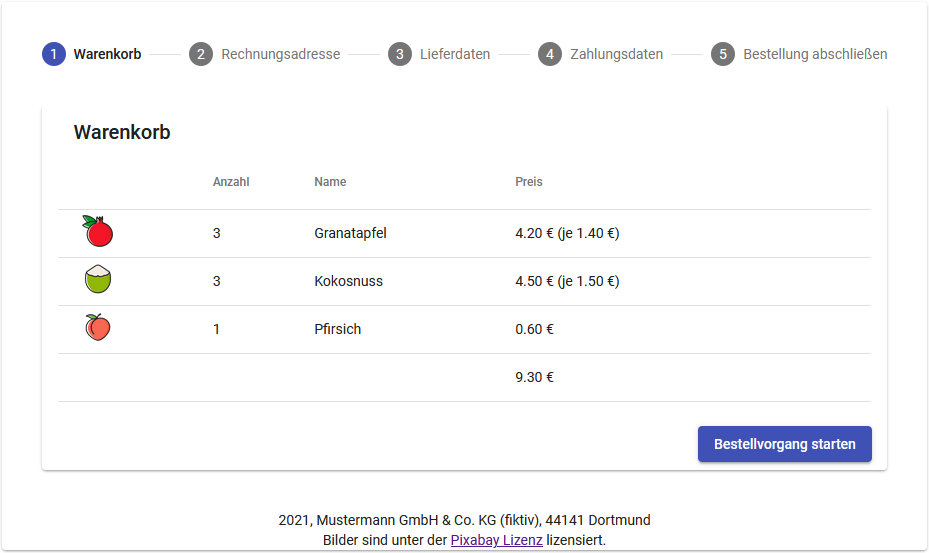
\includegraphics[width=0.75\linewidth]{img/04_erstellung-poc/demoanwendung_vorstellung_01-warenkorb.png}
	\caption{Demoanwendung: Startseite \enquote{Warenkorb}}
	\label{fig:demoanwendung_vorstellung_01-warenkorb}
\end{figure}

\begin{figure}[H]
	\centering
	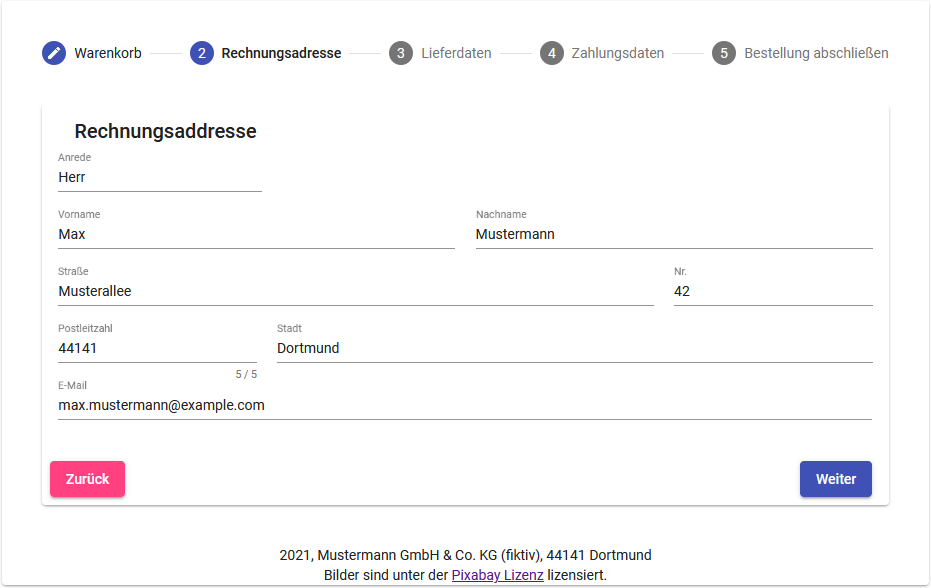
\includegraphics[width=0.75\linewidth]{img/04_erstellung-poc/demoanwendung_vorstellung_02-rechnungsadresse.png}
	\caption{Demoanwendung: Seite \enquote{Rechnungsadresse}}
	\label{fig:demoanwendung_vorstellung_02-rechnungsadresse}
\end{figure}

\begin{figure}[H]
	\centering
	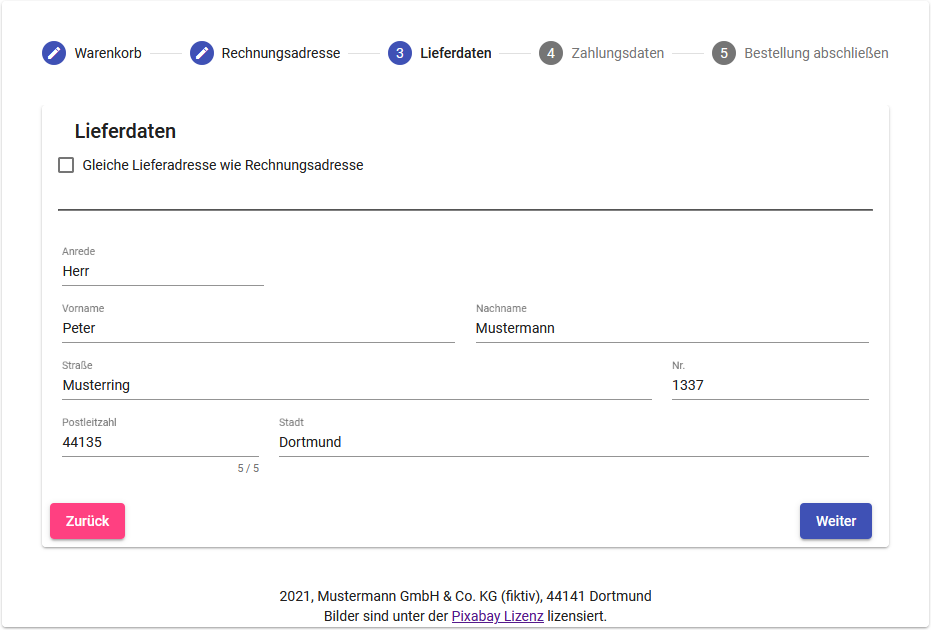
\includegraphics[width=0.75\linewidth]{img/04_erstellung-poc/demoanwendung_vorstellung_03-lieferdaten.png}
	\caption{Demoanwendung: Seite \enquote{Lieferdaten}}
	\label{fig:demoanwendung_vorstellung_03-lieferdaten}
\end{figure}

\begin{figure}[H]
	\centering
	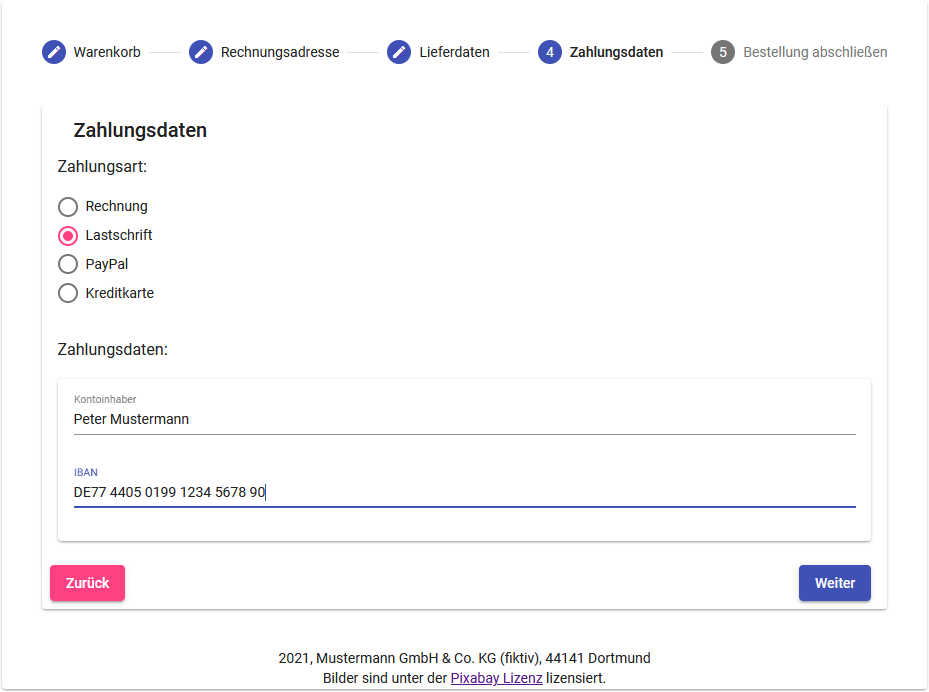
\includegraphics[width=0.75\linewidth]{img/04_erstellung-poc/demoanwendung_vorstellung_04-zahlungsdaten.png}
	\caption{Demoanwendung: Seite \enquote{Zahlungsdaten}}
	\label{fig:demoanwendung_vorstellung_04-zahlungsdaten}
\end{figure}

\begin{figure}[H]
	\centering
	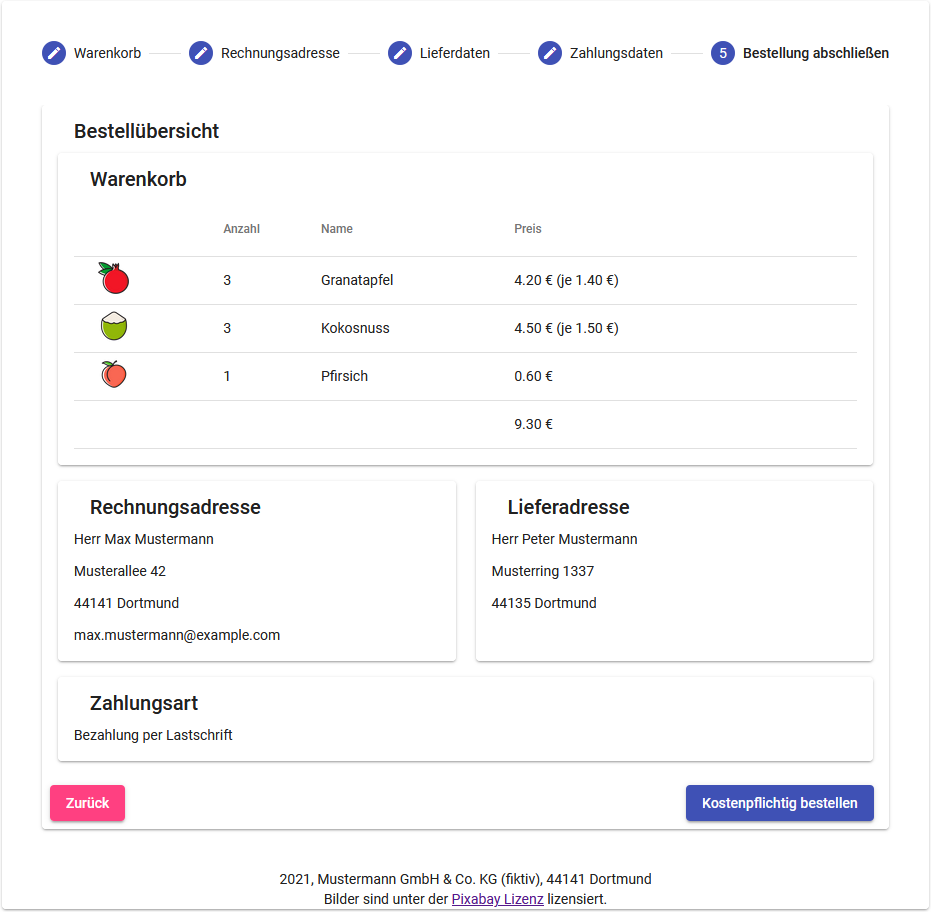
\includegraphics[width=0.75\linewidth]{img/04_erstellung-poc/demoanwendung_vorstellung_05-bestelluebersicht.png}
	\caption{Demoanwendung: Seite \enquote{Bestellübersicht}}
	\label{fig:demoanwendung_vorstellung_05-bestelluebersicht}
\end{figure}

\begin{figure}[H]
	\centering
	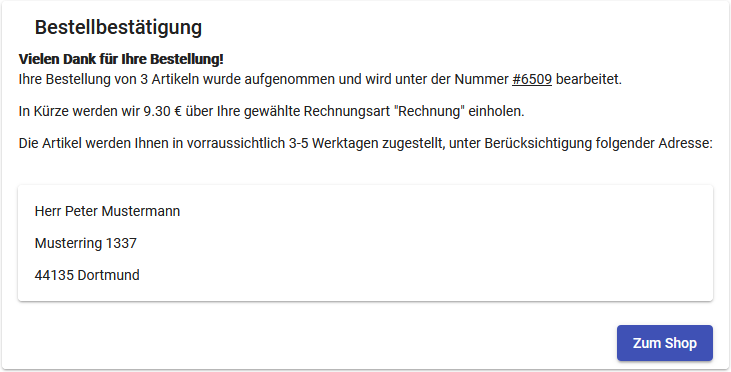
\includegraphics[width=0.75\linewidth]{img/04_erstellung-poc/demoanwendung_vorstellung_06-bestellbestaetigung.png}
	\caption{Demoanwendung: Finale Seite \enquote{Bestellbestätigung}}
	\label{fig:demoanwendung_vorstellung_06-bestellbestaetigung}
\end{figure}

\subsection{Backend}

\begin{figure}[H]
	\centering
	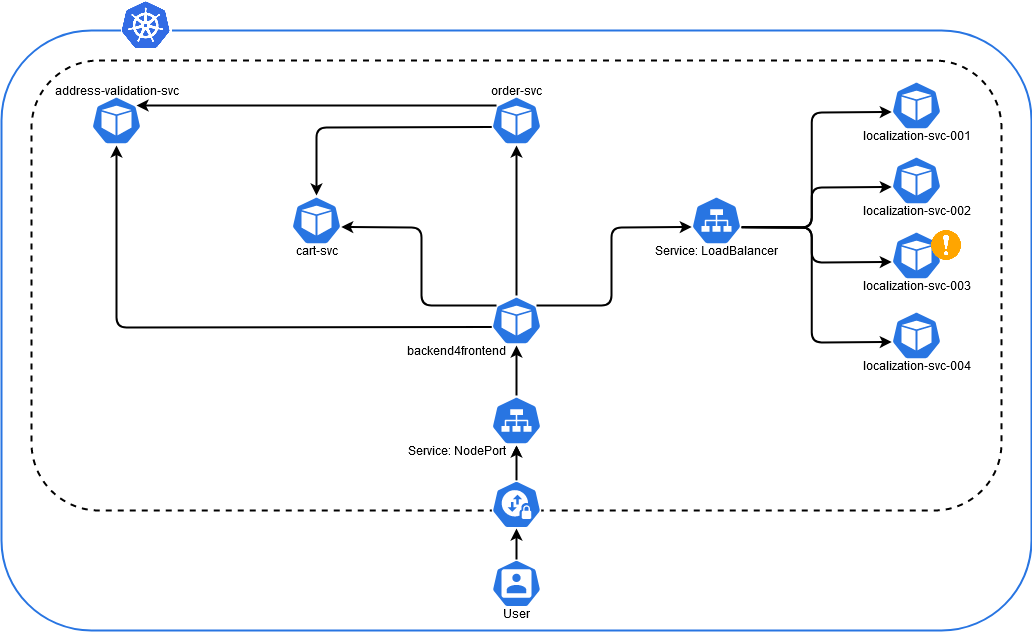
\includegraphics[width=1.0\linewidth]{img/04_erstellung-poc/demoanwendung_k8s-deployment.png}
	\caption{Demoanwendung: Kubernetes-Architektur-Diagramm, Quelle: Eigene Darstellung}
	\label{fig:demoanwendung_k8s-deployment}
\end{figure}